\documentclass[runningheads,a4paper]{llncs}
\usepackage[utf8]{inputenc}
\usepackage[english]{babel}
\usepackage{pdfpages, titling}
\usepackage{array, float}
\usepackage{multicol, booktabs}
\usepackage{cite, tablefootnote}
\usepackage{graphicx, caption, subfigure, wrapfig}
\usepackage{listings}
\usepackage{geometry}
\usepackage{color}
\usepackage{mathtools, braket}
\usepackage{amssymb}
\usepackage[nottoc]{tocbibind} % references in the toc
\usepackage{etoolbox}
\geometry{includeheadfoot, margin=2.54cm}

\usepackage{footnote}
\makesavenoteenv{tabular}
\makesavenoteenv{table}

\usepackage{textcomp}
\usepackage{minted}
\usepackage[hidelinks]{hyperref}
\graphicspath{{Pictures/}} % Specifies the directory where pictures are stored/

\newcommand{\vect}[1]{\boldsymbol{#1}}
\renewcommand{\subtitle}[1]{
  \posttitle{
    \par\end{center}
    \begin{center}\large#1\end{center}
    \vskip0.5em}
}

\author{Jaro Camphuijsen (jcn690), Rahiel Kasim (rkm700), Jan Westerdiep (jwp800)}
\date{\today}
\title{Expedia: Personalised sorting using Learning To Rank algorithms}
\subtitle{Databeestjes - Group 091}
\begin{document}
\maketitle

\section{Introduction}
The online travel agency Expedia started a competition on Kaggle to make a 
recommender system for hotels -- a model that predicts the rating users would give 
to a hotel. The model can be used to present users results relevant to their 
query: the hotels sorted by rating, from high to low. Better models lead to 
better rankings. And better rankings are of interest because users spend less 
time finding the hotel they want. The competition has ended,\cite{kaggle:expedia} 
and the results were published. In this report we will reveal how our own ranking 
model was formed.

\subsection{Outline of this work}
We will start by defining the scoring metric, and will then look at the work of 
prominent Kaggle contestants. We will then discuss our explorations of the data 
set. After this, we will explain our selection of features, which then leads to 
a discussion on the chosen models. We will finalize by reflecting on our work, 
and looking at ways to improve.

\subsection{Scoring metric}
This competition is different from standard Kaggle competitions, in that we are 
trying to predict a rank rather than a class (classification) or some numeric 
value (regression). The scoring metric reflects this; we will therefore give it 
some attention.

Scoring is done via the Normalized Discounted Cumulative Gain metric (NDCG), often used 
in these learning to rank problems. The term \emph{relevance} is integral to this 
metric. In our case, each hotel is either \emph{booked} (having a relevance of 5), 
\emph{clicked} (with a relevance of 1), or none (in other words, irrelevant). 

First, we define the $\text{DCG}_k$ as:
\[
	\text{DCG}_k = \sum_{i=1}^k \frac{2^{\text{rel}_i} - 1}{\log_2(i+1)}
\]
where $\text{rel}_i$ is the relevance score of the hotel placed at rank $i$. The 
value $k$ acts as a truncating parameter: ranks higher than $k$ will not be used.

As an example, let us say we have $k=5$ hotels ranked, with 
$\text{rel} = (1,5,1,0,0)$.  This means that the user booked the hotel ranked at 
position 2, clicked those at 1 and 3, and did nothing with those at 4 and 5. The 
score for this ranking is then
\[
  \text{DCG}_5 = 
    \frac{2^1-1}{\log_2(2)} + \frac{2^5 - 1}{\log_2(3)} + \frac{2^1 - 1}{\log_2(4)} + 
    \frac{2^0 - 1}{\log_2(5)} + \frac{2^0 - 1}{\log_2(6)} = 
    \frac{1}{1} + \frac{31}{\log_2(3)} + \frac{1}{2} + 0 + 0 \approx 21.059.
\]
We see that although both hotel 1 and 3 were clicked, the added value of 3 
towards $\text{DCG}_5$ is only half that of hotel 1. In fact, this added value 
decreases logarithmically in the position, as we can see from the definition.

Of course, we could have scored higher. By swapping hotels 1 and 2, we get a 
relevance vector $\text{rel} = (5,1,1,0,0)$, which yields a $\text{DCG}_5$ of 
$33.596$. In fact, this value is the highest possible; we call this value the 
\emph{ideal DCG} or $\text{iDCG}_5$. The NDCG can now be derived to be
\[
\text{NDCG}_k = \frac{\text{DCG}_k}{\text{iDCG}_k}.
\]
We see that this must always be a value between zero and one. In our case, the 
$\text{NDCG}_5$ value would be around $0.62$.

\section{Related Work}
\label{sec:relwork}
% Your task is to predict what hotels properties listed as a result of a hotel search a user is most likely to click on. Of course, more people have worked on such predictions. Can you find some other people that have tried to make such predictions (e.g. from the Kaggle competition)? And what have they used as most prominent predictors? Have other people that participate in the competition mentioned anything about their approaches? Please spend a couple of paragraphs on this topic (i.e. related work) in your report.
Because this dataset was used in a public online competition, there is a lot of 
information available on the strategies of contestants. In addition to the top-5 
of this Kaggle competition, we found a few others from which we will gather knowledge.

The highest score was achieved by Micheal Jahrer and Andreas Toescher of Opera 
Solutions.\cite{wind} They used a LambdaMART model and got a score of \textbf{0.54075}. 
They used all available numeric features of the test data, and constructed new 
features like the average, standard deviation and mean of all numeric features 
per hotel. These should reduce noise from individual data points in these features. 
The new features were calculated using the training and test data. 
They were disqualified for not complying with the rules.\footnote{Opera Solutions, 
  the company for which the two contestants worked at the time, provides insights 
  into large datasets -- exactly what this Kaggle competition is about. We think 
  that they were not willing (or not allowed) to give up their proprietary code 
  in exchange for the first place.}

Owen Zhang took the 2nd place with a score of \textbf{0.53984} using an ensemble 
of 26 Gradient Boosting Machines (GBM). In addition to the original features of 
the dataset, he introduced composite features like \verb|price_diff_from_recent|, 
the difference between the (current) hotel price and the historical price, and 
\verb|price_order|, the order of the price (cheapest first) in the same \verb|srch_id|. 
He remarked that the most important features were estimated position\footnote{To 
convert categorical features into numerical features so they can be used in a gradient boosting machine, one can use an ``expected feature" calculation where in the training set for all instances of the same 
category we calculate the average score (booked/clicked) of this category. We 
can then do this for all categories which gives us a numerical feature instead of the original categorical. The 
estimated position uses such an expected feature calculation for the property ID, 
the destination ID and the target month, then these so called positions are averaged together with the position of the same hotel in the 
same destination in the previous and next search.}, price and location desirability.\cite{kaggle:presentations} 

Jun Wang got the 3rd place with a score of \textbf{0.53839}. He also used a 
LambdaMART model. He thought that users dislike hotels with missing data, so he 
modeled this by imputing the missing values with the worst case scenario: negative 
values. He employed feature normalization because some features may depend on certain other features, like the market in a particular country, hotel price, month of booking. For example, some high priced hotel may be booked relatively less often in summer because the guests would be more outgoing and give less about luxury while they prefer a better hotel in winter because they spend a lot of time inside. Normalizing the price of hotels per month may in this case result in a better training since it gives you the relative booking rate due to price for each month separately normalized. Jun Wang also recommended removing 
redundant features so they will not interfere with the model as this enhances noise and slows the training down.

The fifth place is occupied by Bing Xu et al.~\cite{bing} with a score of 
\textbf{0.53102}. They used as individual models a linear model, random forests, 
a factorization machine and gradient boosting machines (GBM). These were combined 
in a LambdaMART ensemble. They made composite features like 
\begin{align*}
  \mathtt{count\_window} &= \mathtt{srch\_room\_count} \times \max(\mathtt{srch\_booking\_window}) + \mathtt{srch\_booking\_window},\\
  \mathtt{total\_fee} &= \mathtt{price\_usd} \times \mathtt{srch\_room\_count}, \\
  \mathtt{starrating\_diff} &= \mathtt{visitor\_hist\_starrating} - \mathtt{prop\_starrating},
\end{align*}

and many more. They do not motivate any of their composite features.
They also split the data, training a different model for each \verb|prop_country_id|, 
reducing training time for the individual models.

Table~\ref{table:winners} is a summary of the models, scores and features of the 
reviewed winners. In addition we have added results from other sources. \cite{kaggle:leaderboard}

\begin{table}
\centering
    \begin{tabular}{ llll }    
    \toprule
    Source                  & Model                 & Score   & Strategy                                        \\ \midrule
    1st place               & LambdaMART            & 0.54075 & Numeric features and numeric avg., mean, median \\
    2nd place               & GBM                   & 0.53984 & Expected position, price, location,             \\
    3rd place               & LambdaMART            & 0.53839 & Normalized features                             \\
    Bing Xu et al.          & LambdaMART            & 0.53102 & Split data by \verb|prop_country_id|            \\ 
    Expedia                 & \textit{Proprietary}  & 0.49748 & \textit{Proprietary}                            \\
    David Wind \cite{wind}  & Logistic regression   & 0.47301 & Outliers: hotels with price $>$ \$10,000 removed\\
    Kaggle Python Benchmark & Random Forests        & 0.40356 & Impute missing values with zeros                \\
    Random order            & Random                & 0.34958 & Random                                          \\ \bottomrule
    \end{tabular}
    \caption{A summary of employed strategies.}
	\label{table:winners}
\end{table}

\section{Exploratory Data Analysis}
% Essentially, this is a subtask that requires you do exploratory data analysis (EDA). Explore the dataset, count, summarize, plot things, and report findings that are useful for your task. Remember that EDA is not necessary done once and then you move on. It might very well be possible that you do some EDA, build some models, then some idea comes up, do some more EDA, modify your model according to what it shows, and so on.

We have a large data set; both the training and testing sets contain a little under 
5M rows each, with 54 training features and 50 testing features.  Each row 
represents a hotel in a search query, so that a group of rows together make up a 
search query. We can group the features into a few categories, namely
\begin{description}
	\item[Search query features] like 
    search ID (integer); 
    date and time of search (datetime); 
    number of rooms (integer); 
    destination country ID (integer); 
    number of people (integer);
  \item[Hotel features] like 
    hotel ID (integer); 
    average rating (integer between 1 and 5); 
    two scores measuring its location desirability (float); 
    whether it is part of a chain or independent (boolean);
    natural log of the average price this hotel was listed as (float);
  \item[Visitor features] like 
    the country of origin ID (integer); 
    mean nightly price this user previously paid (float); 
    mean star rating of hotels previously slept in (float);
  \item[Hotel-query features] like 
    listed price (float); 
    whether it was explicitly flagged as being a promotion (boolean); 
    the distance from visitor to hotel (float);
    10-log of probability this hotel will be clicked from a Google search (float);
  \item[Competitor features] describing the relative listed price for this hotel 
    (both boolean and float), for its eight largest competitors.
\end{description}

These hotels were listed in either random order or as ranked by their own 
algorithm, which is another boolean feature. In the training set, we have another 
four features:
\begin{description}
	\item[Position;] an integer between 1 and 38 showing its position on the Expedia results page;
    \item[Click and booking;] two booleans checking whether a user clicked resp.~booked this property;
    \item[Gross Booking USD;] a floating point number signifying the total cost of this transaction.
\end{description}
Of these training features, the click and booking booleans are the most important; 
these define the relevance used in the final scoring metric and are integral to 
training models that work well. 

To get a feeling for what we are working with, we will now discuss a few highlights
of our explorations. In fact, a lot of the exploration was already done \emph{for us}: 
the Kaggle forum of this competition contains a lot of valid and interesting points.
For instance, the price of a hotel can either be a nightly price, or for the entire
booking in total. The latter is actually a combination of two features, the nightly price and the \verb|length_of_stay|. Each hotel decides for itself which of these it shows on Expedia, so the price becomes an unreliable feature. It would be good to distinguish total stay prices and convert them to nightly prices to get a proper price feature.\footnote{One way we propose to do this is to find for each property, for each length of stay, the mean price (this is possible with Pandas using \texttt{df.groupby(["prop\_id", "length\_of\_stay"])["price\_usd"].mean()}), yielding a sparse matrix. This matrix could be interpolated to yield a full matrix. For each property id separately, one can then compute some kind of ``mean difference''; a positive value implies a nightly rate, whereas a negative value implies a flat per-booking rate.}

\subsection{Time frame}
\begin{figure}[h]
	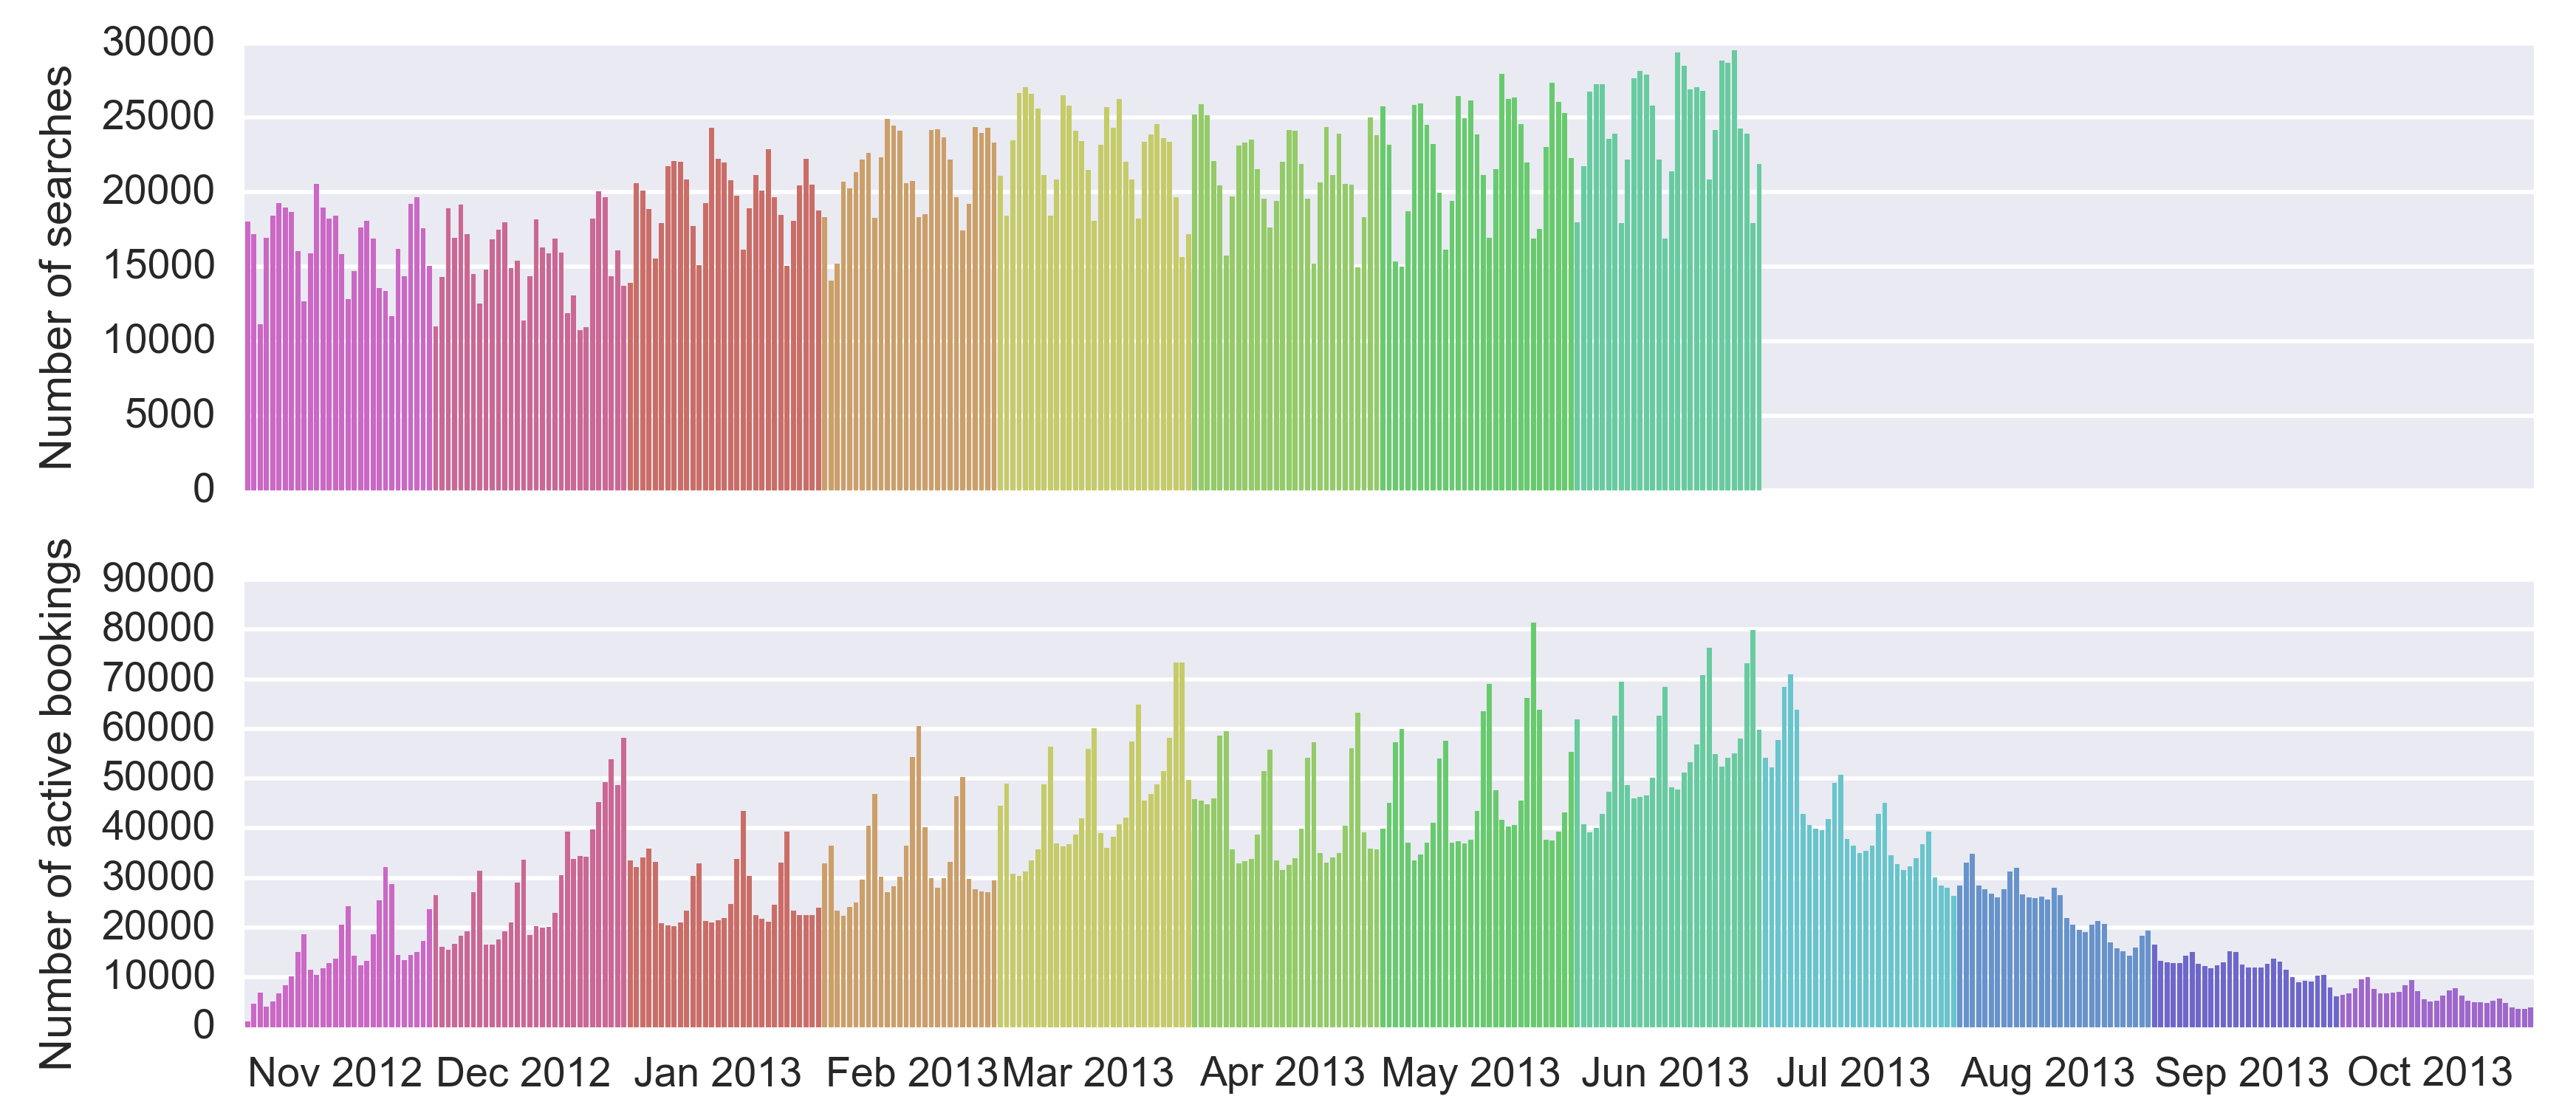
\includegraphics[width=\linewidth]{Pictures/dateplot.png}
    \caption{Visualisation of the data extracted from three temporal features. Top: the total number of searches per day; bottom: total number of bookings active per day.}
    \label{fig:dates}
\end{figure}
We quickly noticed that the \verb|date_time|, \verb|srch_booking_window| and 
\verb|srch_length_of_stay| together determine on which nights a hotel was booked.  
We visualised this, together with the number of daily searches, in Figure~\ref{fig:dates}. 
A few things immediately become clear: firstly, we only have Expedia searches between 
November 2012 and June 2013. The actual hotel stays were in a much larger time 
frame, mostly because people tend to book in advance. 

Moreover, in both graphs we see a very evident weekly trend; people tend to search 
less during weekends, but stay in hotels more.  Other notable things we see from 
this graph is that people tend to search less during Christmas, but travel more; 
there is a slight peak around February 14 (Valentine's Day); there are larger peaks around Easter 
and the summer holidays in June. After June 2013, we are less sure about the things 
we see, as no more new bookings are tracked.

\subsection{Outliers}
The dataset is not preprocessed and therefore contains a significant number of 
outliers. Figure~\ref{fig:outliers} shows, for a select set of features, a 
box-plot of the data. 

What we immediately see is that a few lines extend all the way to the left; this 
means that a sizable chunk (the lowest 25\% of the non-NaN values, in fact) are 
below $10^{-4}$; this is attributed to the fact that there are just a lot of zeros 
in the booking window, for instance.

We see that a lot of these features have wide-spread outliers (the black dots to the right of the third quartile whiskers): 
the price of a hotel, for instance, is between $\$0.01$ and \$10,000,000; there 
can be up to a 1,000,000\% difference between the price of a hotel on Expedia 
versus a competitor; the destination is between $10$ metres and 10,000 kilometres from the original location. 
In our feature engineering phase, we will make sure to remove those features or rows with many outliers.
\begin{figure}[h]
	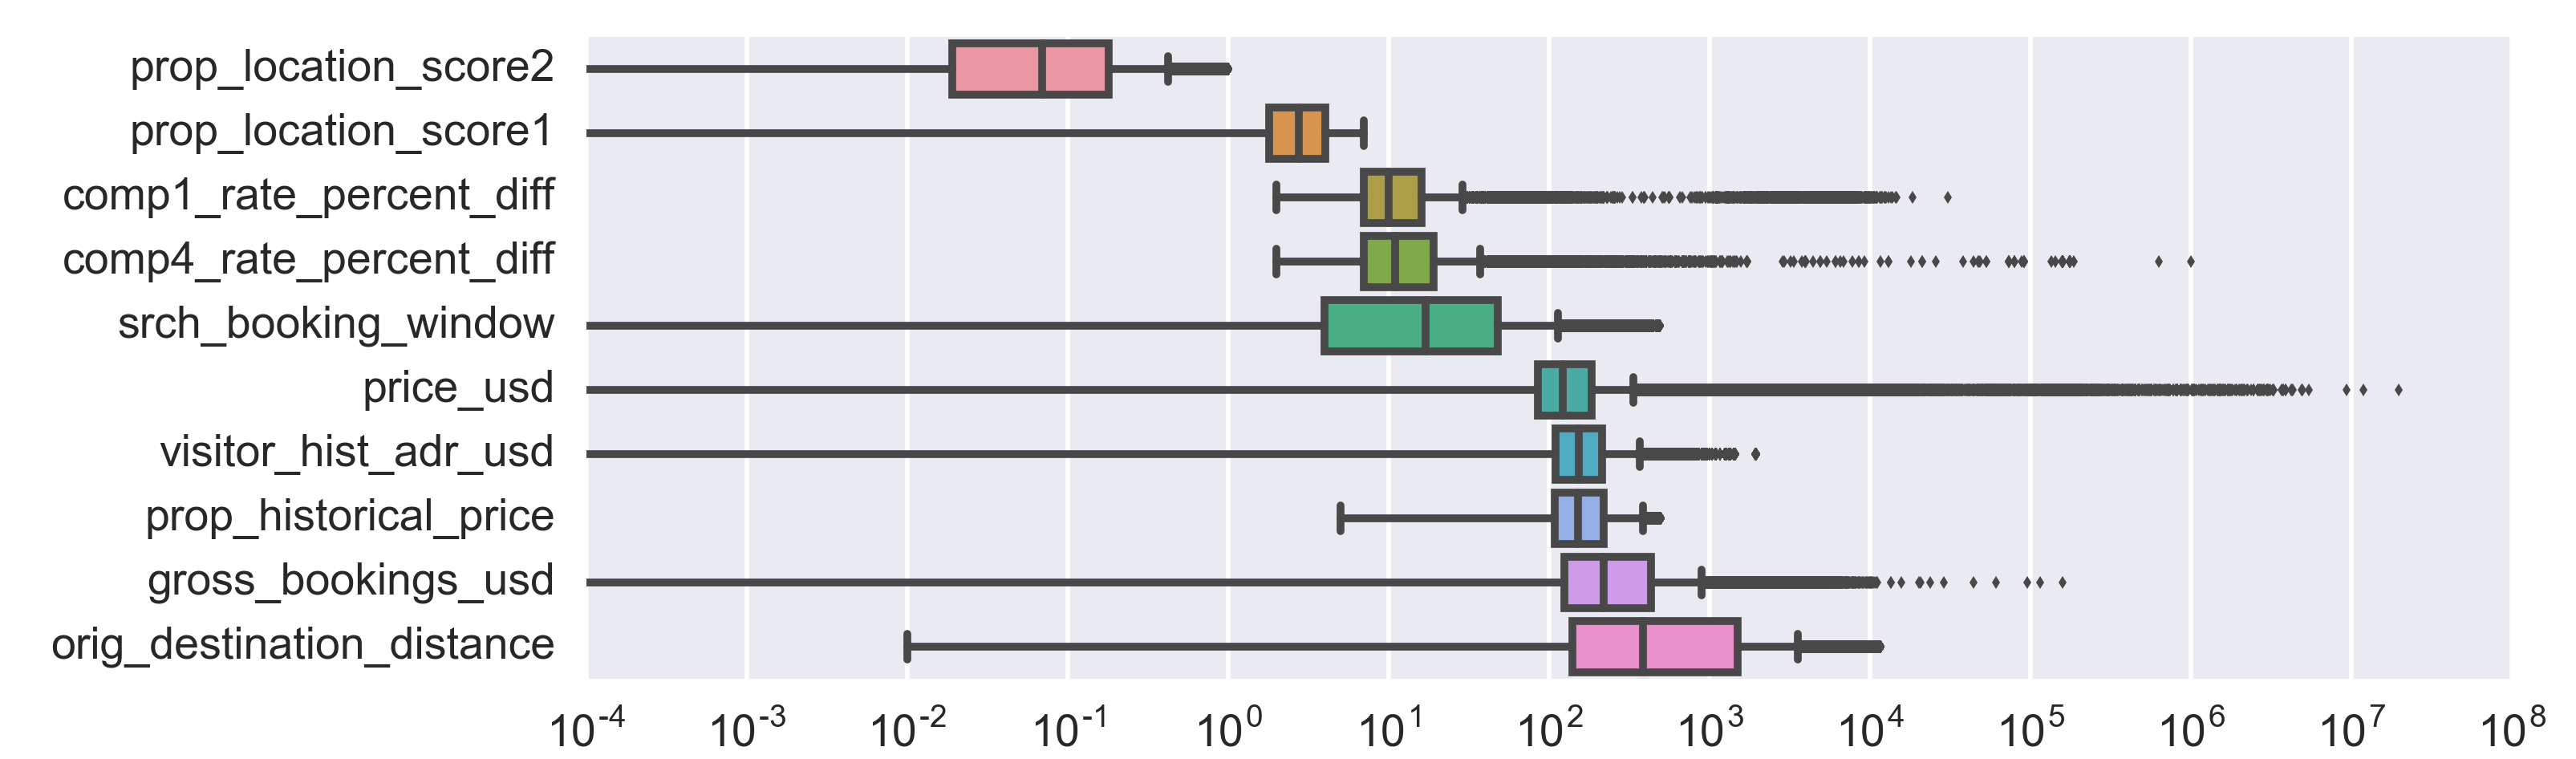
\includegraphics[width=\linewidth]{Pictures/outliers.png}
    \caption{The distribution of the values for a selected set of features.}
    \label{fig:outliers}
\end{figure}

\subsection{Missing Data}
Again, this is a real dataset, so we ca not expect every cell to be filled. For instance, some users are first-time Expedia bookers, so that the \verb|visitor_hist_adr_usr| -- the mean historical price for this user -- must be null. Moreover, if a hotel is \emph{only} available on Expedia, and not on any of its competitors, all these competitive features must be null as well. Figure~\ref{fig:barplot} shows the percentage of missing values for each feature. We see that exactly the previously mentioned features are lacking; moreover, historical data on properties is in some cases missing.\footnote{It was found on the competition forum \cite{kaggle:forums} that a value of $0.0$ for \texttt{prop\_log\_historical\_price} signifies a missing data point as well.}

\begin{figure}[h]
	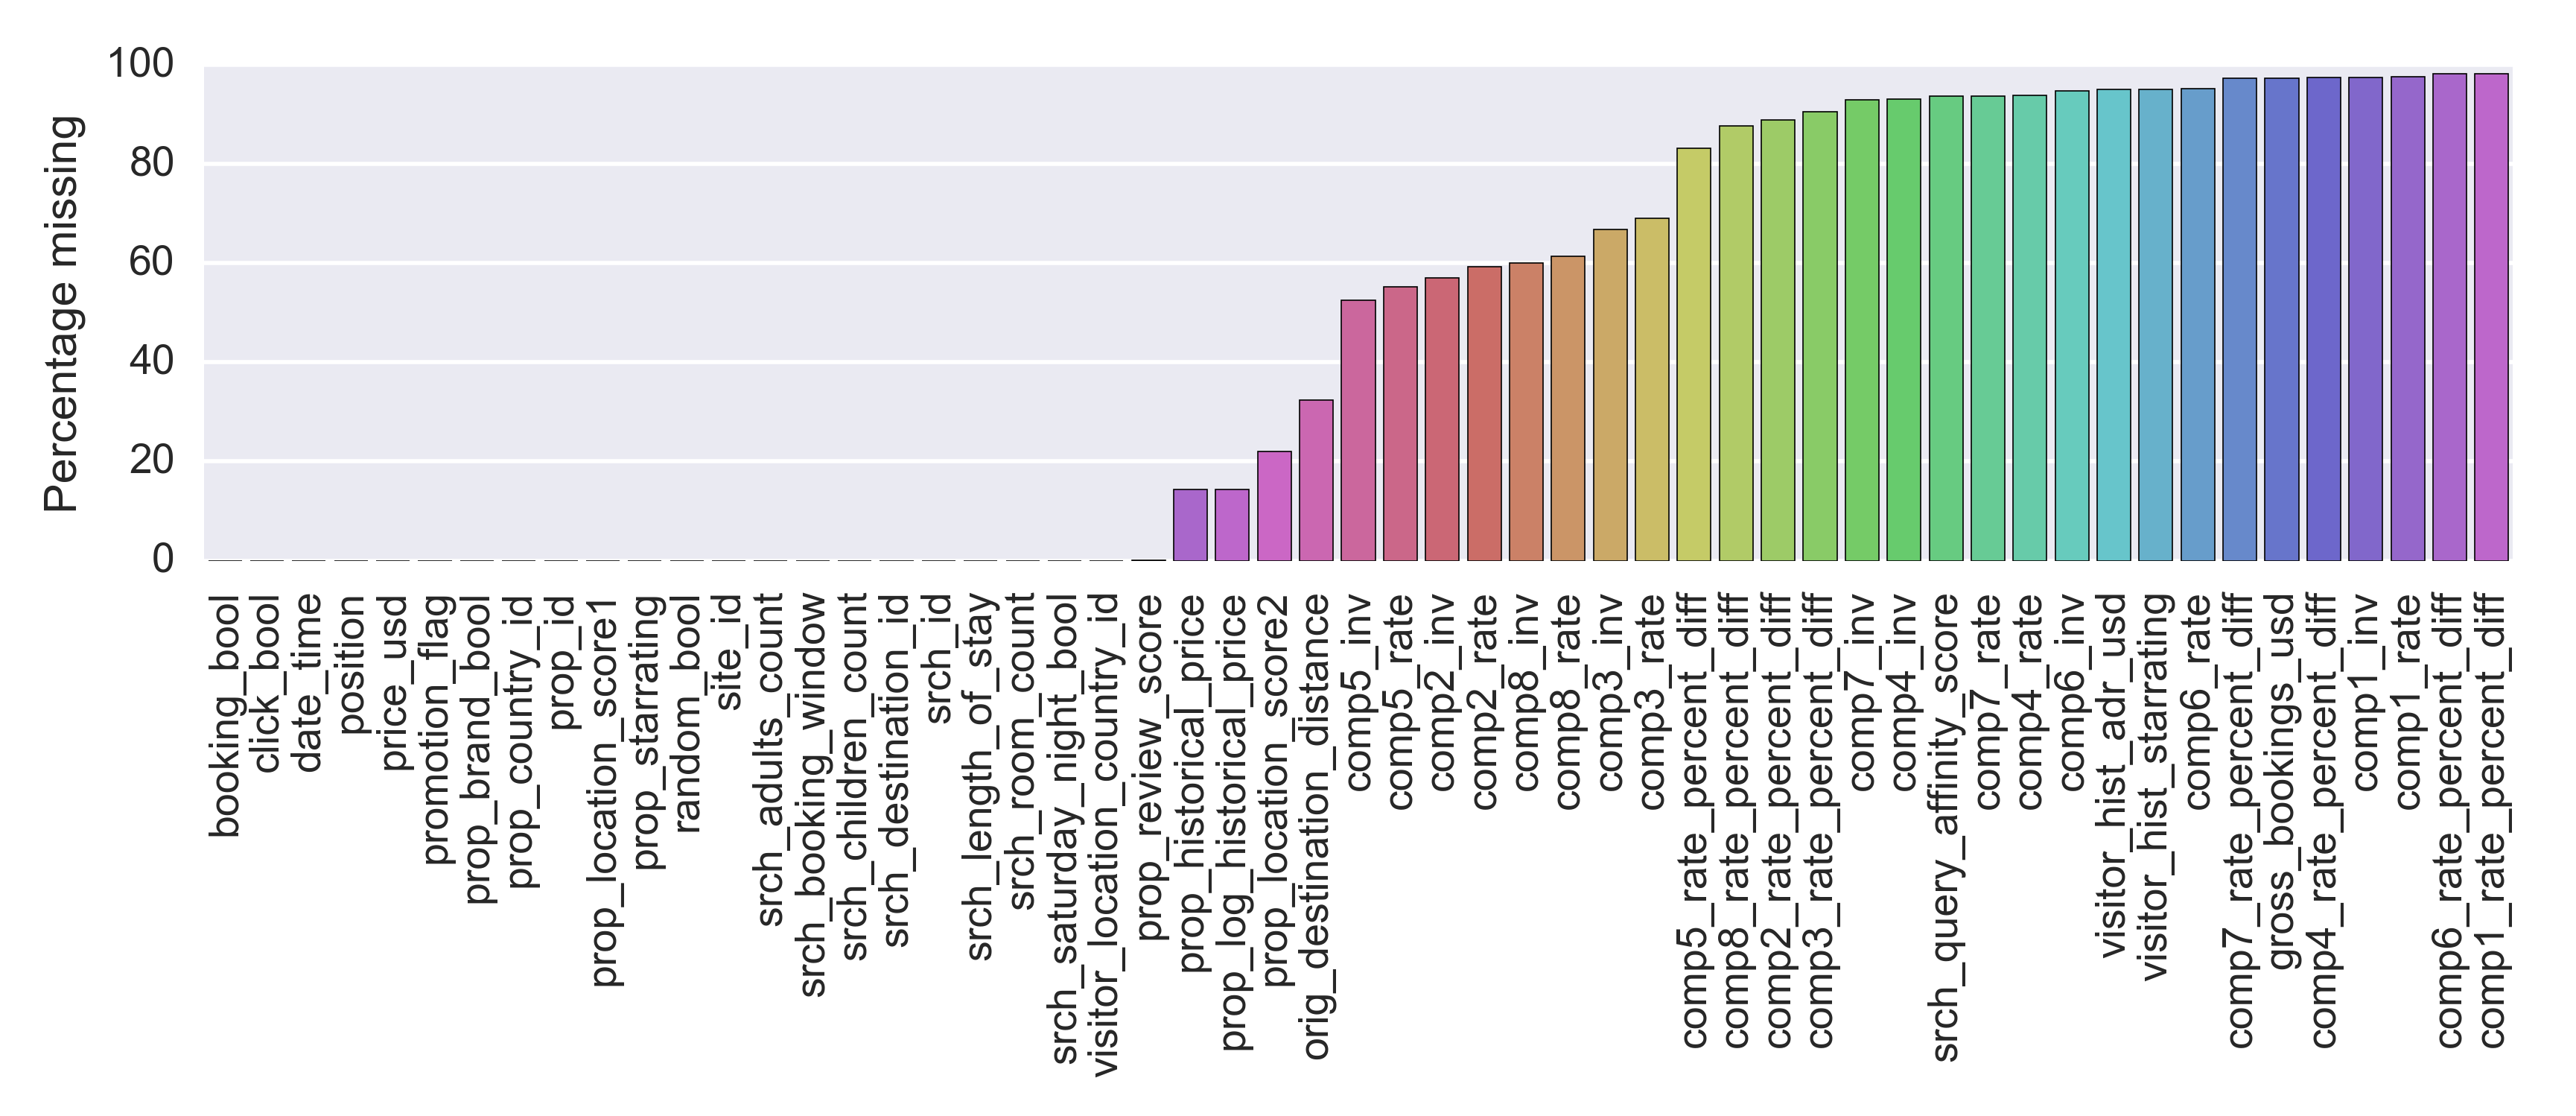
\includegraphics[width=\linewidth]{Pictures/barplot.png}
    \caption{Percentage of data missing for each feature in the original training dataset.}
    \label{fig:barplot}
\end{figure}

\section{Feature Engineering}

As Domingos mentions in his review paper on machine learning \cite{domingos}, easily the most important part of any machine learning project is the feature engineering. There is however little to no theory on how to do it well. We will simply have to experiment, train a model and evaluate the results. More cost-effective is to copy successful strategies from previous work, this was our primary guideline. Let us start by describing the features we have used.

We employ roughly three types of features:
\begin{description}
  \item[Original features,] making sure to handle missing values correctly;
  \item[Derived features] are made by transforming existing features;
  \item[Averaged numerical features] which aggregate data on a larger set of rows.
\end{description}

\subsection{Original Features and missing data}
Since many of the original features cover only small part of the data set -- an 
insight found by examining Figure~\ref{fig:barplot} -- we have to decide how to 
handle missing values.\footnote{Further examination showed that in fact most of the
  columns did not miss any data at all. We see in the figure a very faint line at 
  \texttt{prop\_review\_score}; this has around 7000 missing values, but everything to the 
  left has none.}

It was our decision to remove all features with more than 50\% missing data, as 
we figured they would have too little discriminative value. This leaves us with
three columns having missing data: the property location score, the distance 
between destination and current location, and the historical review score.

As mentioned in \textit{Related Work}, it was found that Jun Wang (3rd place) imputed missing data with the 
\emph{worst case scenario}. For instance, we filled missing historical hotel ratings with a value of $-1$; after all, a negative rating is as bad as it gets.

In \cite{bing}, missing values were handled slightly differently: for 
instance, the second property location score -- indicating the desirability of 
the property location -- was imputed by taking the first quartile value of the
properties in the same country as the current property.\footnote{This is slightly
  hard to explain, but is easily implemented using Pandas\cite{pandas} by means
of a \texttt{df.groupby("prop\_country\_id")["prop\_location\_score2"]} command.}

We experimented with the two variants and ultimately decided to use both: for the
two location-based columns, we used the quartile method; for the historical review 
score, with only a few missing data points, we used the worst-case scenario method.

This leaves us with a grand total of 19 original features, outlined below:
\begin{multicols}{3}   
    \noindent
    \verb|site_id| \\
    \verb|visitor_location_country_id| \\
    \verb|prop_country_id| \\
    \verb|prop_starrating| \\
    \verb|prop_review_score| \\
    \verb|prop_brand_bool| \\
    \verb|prop_location_score1| \\
    \verb|prop_location_score2| \\
    \verb|price_usd| \\
    \verb|promotion_flag| \\
    \verb|srch_destination_id| \\
    \verb|srch_length_of_stay| \\
    \verb|srch_booking_window| \\
    \verb|srch_adults_count| \\
    \verb|srch_children_count| \\
    \verb|srch_room_count| \\
    \verb|src_saturday_night_bool| \\
    \verb|orig_destination_distance| \\
    \verb|random_bool|
\end{multicols}

\subsection{Derived Features}
A few of the original features are in principle usable, but in a format not fit
for our model to train on. For instance, the exact booking moment might affect a
user's behaviour; they might make decisions differently on weekends than on 
Wednesdays, or might prefer a more expensive hotel early in the month, when they
still have money. We expected that the exact timestamp would not work well as a feature because of its huge range: every second from the start, to the end of the data. With the previous considerations in mind, we decided to split the \verb|date_time| into four features, each with smaller ranges: the month, week, hour, and the day of the week. These four features replaced \verb|date_time|. This was also the approach of one of the contestants. \cite{wind}

The feature \verb|prop_log_historical_price| was originally saved as a logarithmic 
scale with natural base,\cite{kaggle:forums} so we converted it to a regular historical price.\footnote{We
  could not find a source explaining the reason behind saving a logarithm, but 
  the feature \texttt{srch\_query\_affinity\_score} is
  also saved logarithmically. It signifies the (estimated) log probability that this 
  hotel will be clicked from a Google search. This feature varies between $-1$ 
  and $-72$, so saving it without a log yields too many leading zeros. In our case
  however, the prices differ not nearly as much -- between 1.6 and 6.2 -- so this can not 
  be the reason.}

We used the \verb|count_window| feature from \cite{bing}, as explained in \S\ref{sec:relwork}. The authors gave no motivation for the feature, we have used it because it worked for them.

\subsection{Averaged numerical features}
\label{sec:avg}
Each row of our dataset contains a few numerical features related to the property
in a specific search query. Because these searches are made over a period of time,
the rating of a property might change between the first and last search. Our model
does however not correct for this time-dependent noise. This, combined with the 
knowledge that we want to rank properties within a search query,
made the (disqualified) winners of the Kaggle competition add some aggregate features. \cite{kaggle:forums}
We recognized this as a good idea and implemented it. Note that these features were computed using the 
\emph{whole} dataset, being the concatenation of train and test.

For each property ID, we determine the mean, median, and standard deviation of the
\verb|prop_starrating|, \verb|prop_review_score|, \verb|prop_location_score1|, and
\verb|prop_location_score2| and add these 12 new features.

\section{Model selection}
The problem at hand can be seen as a regression problem by training on the \verb|click_bool| and \verb|booking_bool| variables, then ranking them in the right order.  However, there are specialised algorithms to rank documents linked to queries. To make it challenging for ourselves, we chose to pursue using -- just as the Kaggle winners generally have done -- such a Learning To Rank algorithm instead.  There are a lot of packages available for doing this; we chose two. The first, RankLib\cite{ranklib}, is widely used and very fast.  The RankPy\cite{rankpy} library provides us with a little more fine-grained control over training, model selection, and testing. The decisive reason for us to use RankPy is however its affiliation with the University of Amsterdam.

Usually, one reserves 20\% of the total training data for model validation; the size and homogeneity of this dataset allows us to reduce this to 10\%,\cite{bing} and we will do so by selecting as validation set all queries with \verb|srch_id| a multiple of ten.  In early test runs we used a subset of the data, but our final models were trained on the entire training set.

\subsection{LambdaMART}
Many of the Kaggle winners used one such Learning To Rank algorithm called LambdaMART, for which a very good self-contained article explaining the history and derivation is available. \cite{burges2010} In this applied course on Data Mining, we will refrain from diving into the details of this algorithm, focusing more on its application. This ensemble method contains many parameters that we can tune, most of them changing the behaviour of the decision trees within it. Because of time constraints, we chose not to play around with the default values \emph{too} much, mostly changing the stopping criteria.

\section{Final Results}
Our final results were gathered on a quad core i7-3770 machine running at 3.4GHz, with 16GB of memory. Scripting was almost exclusively done in Python, with the Pandas library \cite{pandas} for feature engineering, SVMRank \cite{svmrank} as an intermediary file handler, and RankPy \cite{rankpy} or RankLib \cite{ranklib} for training.  The size of the dataset required us to tread carefully: simply looping over every row in the dataframe to compute the weekday was already enough to bring the machine to a grinding halt, and having multiple copies of the dataframe in memory resulted in swapping and laggy behaviour.

It takes our machine about an hour to generate all the necessary features and write everything to disk. Depending on the algorithm and convergence rate, training takes between 1 and 8 hours per run. We suspect that both libraries do not retrain the final model with both train and validation data, but seeing as they are plug-and-play, we can not know for sure without diving into the nitty gritty. It does not matter too much, as the validation set is just 10\% of the 5 million training rows.

\subsection{Validation Score}
We managed to fully train three models scoring higher than the Expedia benchmark (cf.~Table~\ref{table:winners}). Two of them were based on the full feature set with different algorithms, the third with a smaller set. We see the validation NDCG@38 as a function of the iteration number in Figure~\ref{fig:valiscore}. We stopped the algorithms manually after 1000 iterations. It shows clear diminishing returns, with a sub-logarithmic progression even. From this we conclude that, although two of the models were still growing in score after 1000 iterations, the added value of letting it run would have been negligible. The third model in purple was stopped early, after 25 disappointing iterations without increase.

\begin{figure}[h]
	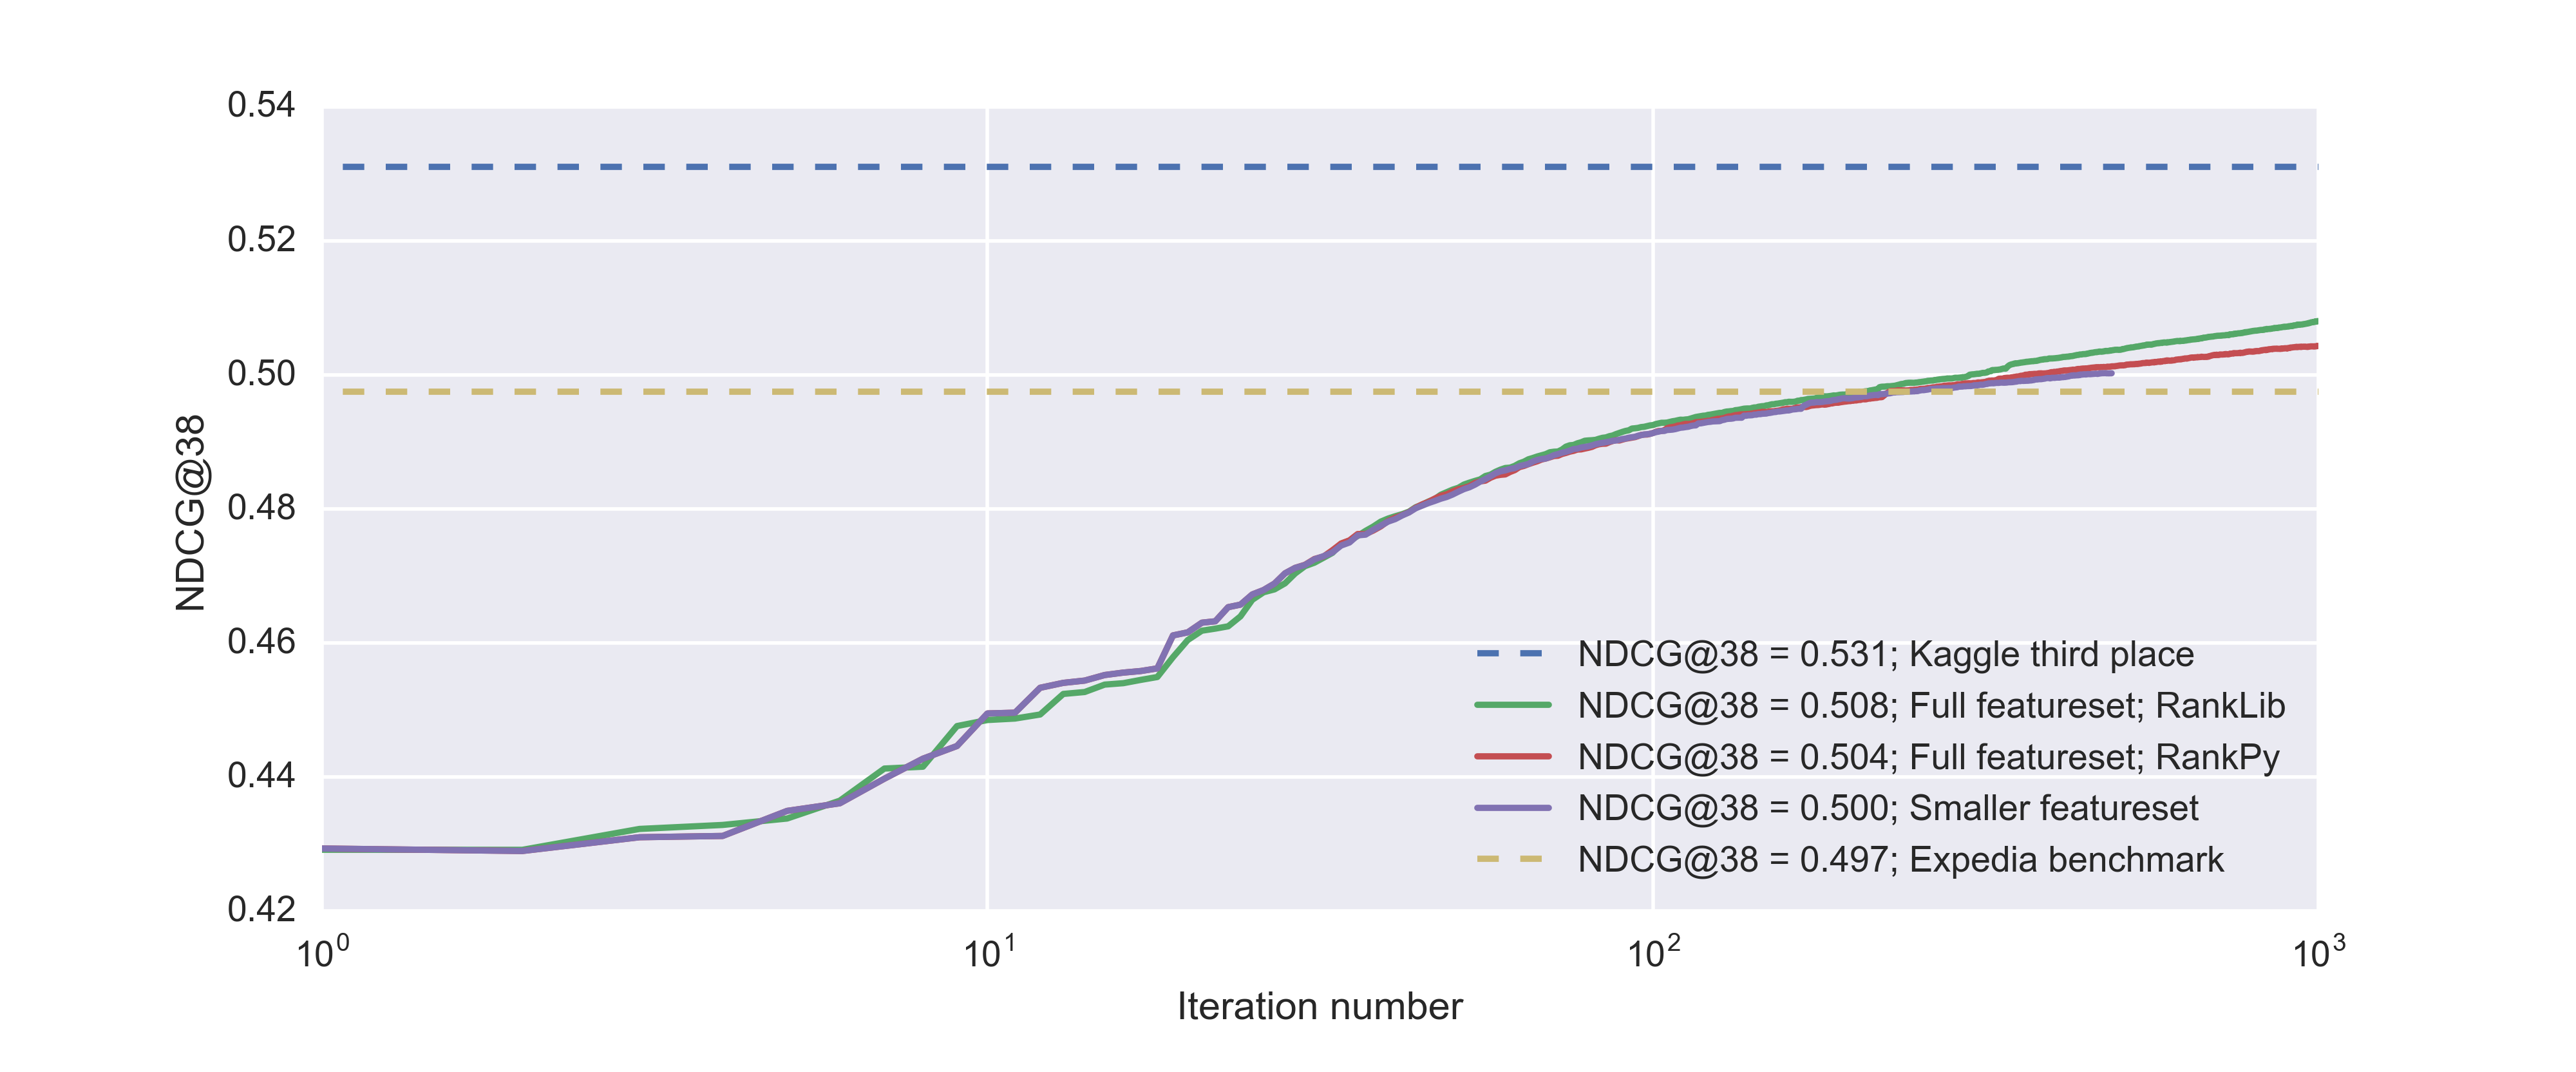
\includegraphics[width=\linewidth]{Pictures/models.png}
    \caption{NDCG@38 score for our different models as a function of the iteration number.}
    \label{fig:valiscore}
\end{figure}

The highest-scoring model in green was trained using RankLib with the LambdaMART algorithm; the second-highest in red was also a LambdaMART algorithm, this time trained with RankPy. The main difference in score can be attributed to the tweaking of the hyperparameters, most notably the \verb|min_samples_leaf| or \verb|mls| parameter, which controls the growth rate of the decision trees by requiring a minimum number of samples within a leaf to branch the decision tree. In the RankPy model, this was set to a very liberal 50 (the default setting), whereas in the RankLib model, we tried a value of 50,000. This was to account for the size of this dataset, resulting in an improvement of 0.004 from \textbf{0.504315} to \textbf{0.508005}.

We wanted to test the claim of Michael Jahrer that adding the averaged features (cf.~\S\ref{sec:avg}) increased the score by 0.2, or equivalently, that removing them would \emph{decrease} it by 0.2 as well. The result is both surprising and disappointing: our model (with the same settings as the LambdaMART RankLib algorithm) still performs quite well (\textbf{0.500229}; in purple, stopped after 490 iterations) without it.

\subsection{Feature Importance}
LambdaMART being a decision tree-based ensemble method, we can easily compute the feature importances. This provides us with insight on possibilities for improvement. See Figure~\ref{fig:importances} for the relative importances of our features. We see that even a categorical feature like \verb|prop_id| accounts for 5\% of its predictive power, and that the standard deviation per hotel generally do nothing. 

We also see that splitting the date helped: while the month, day and hour do not contribute much, the day of the week (simply \verb|day| in the figure) has a higher importance than the hotel's rating (\verb|prop_starrating|). 

The noise-canceling effect of the averaged numerical features from \S\ref{sec:avg} can be seen: both the mean and median of the \verb|prop_starrating| perform better than the original feature itself. For \verb|prop_location_score1| we see the median/mean tagging along closely.

However, the most astonishing part is that from the top 6 most important features, 3 are (some variation of) the second location score, making up a total relative importance of around 34\%. This had us scratching our heads for quite some time, until we found on the Kaggle forums that Owen Zhang, the official winner of this competition, had stated: ``Just to get you started, the variable \verb|prop_location_score2| seems to be a good feature.'' \cite[Topic 6177]{kaggle:forums}. Combining this with the quote from the officious winner Michael Jahrer, referring to the method explained in \S\ref{sec:avg}: ``We got the biggest improvement by adding the avg per \verb|prop_id| (0.51 to 0.53).\cite[Topic 6228]{kaggle:forums}''. We see that it is possible that this feature works very well.

\begin{figure}[h]
	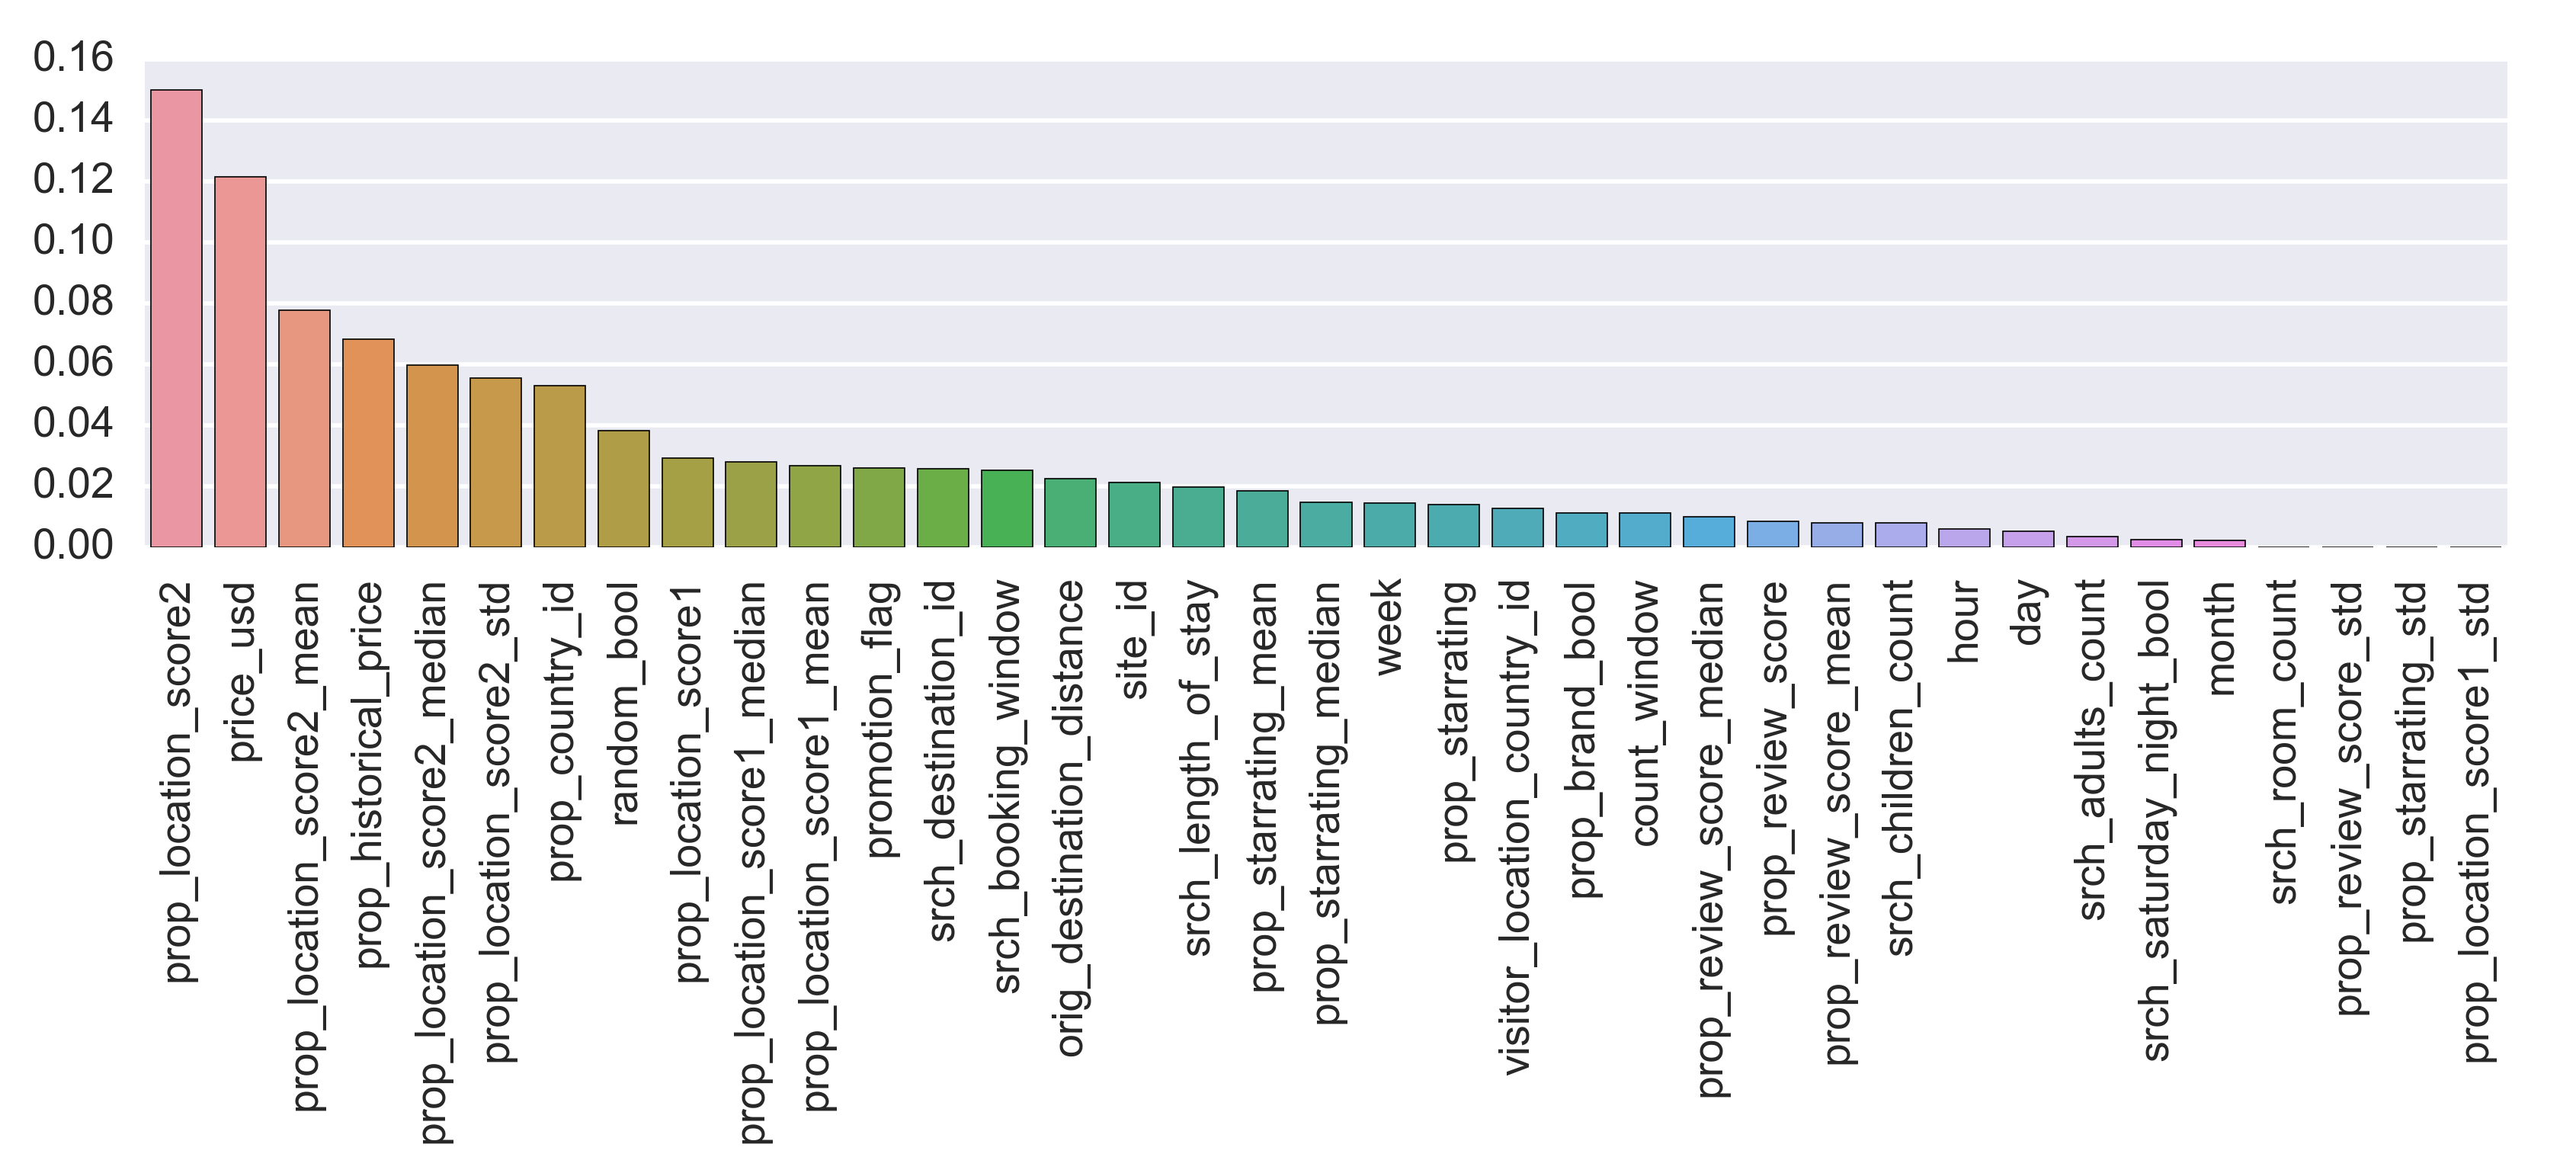
\includegraphics[width=\linewidth]{Pictures/feature_importances.png}
    \caption{Relative feature importances for a trained LambdaMART model.}
    \label{fig:importances}
\end{figure}

\section{Discussion}
Our main strategy in this assignment was to ``learn from the best'' and combine the decisions, both in choosing a model and in feature engineering, the winners had made. This worked impressively well: we were amazed by the results we got. We learned that you must not ignore previous related work; our final models even beat the Expedia benchmark, which in itself is quite surprising.

This assignment has taught us a lot about working with \emph{big data}. We were lucky to have a machine with sufficient memory to load our dataset, but we had to be very careful in how we operated over the data. We were used to naively loop (multiple times) over all the data to perform some operation, but now the data was so big that this would take a considerable amount of time. This lead us to learn how to use the Pandas library to efficiently manipulate data.

Playing around with and learning something about LTR algorithms was also enlightening. Here again, we noticed how algorithmic complexity can make all the difference; Random Forest models trained within the order of minutes, whereas our final model took a full work day to train.

Finally, we learned to appreciate the exploratory data analysis phase. Our graphing skills improved and some figures helped in taking decisions. For instance figure \ref{fig:barplot} told us which features to exclude when training the model.

\subsection{Future work}
We spent some time figuring out how to efficiently make new features, and were relieved when it worked. We could have easily added more derived features, for example those mentioned in \cite{bing}, but were restricted by time.

As discussed in \S\ref{sec:relwork}, the prize winner mentioned his estimated position as the most important feature.  We recommend looking deeper into it and implementing it. More generally, we recommend having more derived features.

Although LambdaMART is an ensemble method in itself, we would have liked to combine multiple well-performing models into one majority-vote ensemble method.

Moreover, RankLib provides a lot of different ranking algorithms, many of which we did not use. Each algorithm has a plethora of different parameters which you can tune using the built-in cross-validation functionality. It also allows one to select a subset of the features. Given more time, this could pave the way towards a top-performant ensemble method.

We conclude with a simple and trivial suggestion to get better results: train the final model on the full data, i.e. without splitting off the validation data. More data should lead to a better model. We already had this in mind, but had no time due to the tardiness of the calculation.

\vfill

\begingroup
\let\clearpage\relax
\bibliography{references}
\bibliographystyle{unsrt}
\endgroup

\end{document}

